% Compilar con XeLaTeX (Overleaf: Menu -> Compiler -> XeLaTeX)
% Logo: subir el logo de la UIS al proyecto con el nombre logo_uis.png (si no existe, se omite)
\documentclass[aspectratio=169, 11pt]{beamer}
\usepackage{fontspec}
\usepackage[english, spanish, provide=*]{babel}
\usepackage{amsmath, booktabs, graphicx}
\graphicspath{{../figs/}{figs/}{./}}

\definecolor{uisverde}{HTML}{3D8B37}
\definecolor{uisoscuro}{HTML}{1F4D1C}
\definecolor{gris}{HTML}{555555}
\usetheme{default}
\setbeamercolor{frametitle}{fg=white, bg=uisverde}
\setbeamercolor{title}{fg=uisoscuro}
\setbeamercolor{structure}{fg=uisverde}
\setbeamercolor{alerted text}{fg=orange!85!black}
\setbeamerfont{frametitle}{size=\large, series=\bfseries}
\setbeamertemplate{navigation symbols}{}
\setbeamertemplate{itemize items}[circle]
\setbeamertemplate{frametitle}{\nointerlineskip
  \begin{beamercolorbox}[wd=\paperwidth, ht=2.4ex, dp=1.2ex, leftskip=0.6cm]{frametitle}
  \usebeamerfont{frametitle}\insertframetitle\hfill
  \IfFileExists{logo_uis.png}{\raisebox{-0.6ex}{\includegraphics[height=3.2ex]{logo_uis.png}}\hspace{0.4cm}}{}
  \end{beamercolorbox}}
\setbeamertemplate{footline}{\hfill\textcolor{gris}{\scriptsize Ríos, Sarmiento · Mecánica Clásica UIS · \insertframenumber/\inserttotalframenumber}\hspace{0.4cm}\vspace{0.2cm}}

\title{¿Hasta dónde sirve el análisis lineal?}
\subtitle{Los troyanos de Júpiter frente a la teoría de pequeñas oscilaciones}
\author{Paola Andrea Ríos Campos \and Juan Diego Sarmiento Villarreal}
\institute{Escuela de Física · Universidad Industrial de Santander\\ Mecánica Clásica · Reto III.1}
\date{18 de noviembre de 2026}

\begin{document}

% 1 ------------------------------------------------------------------
\begin{frame}[plain]
\IfFileExists{logo_uis.png}{\begin{center}\includegraphics[height=1.4cm]{logo_uis.png}\end{center}}{}
\titlepage
\end{frame}

% 2 ------------------------------------------------------------------
\begin{frame}{El problema}
\begin{columns}[c]
\column{0.5\textwidth}
\begin{itemize}
\item Asteroides que comparten la órbita de Júpiter, $\sim60^\circ$ delante ($L_4$) y detrás ($L_5$).
\item Teoría clásica: \textbf{pequeñas oscilaciones} alrededor de $L_4$.
\item Pero los reales ocupan \alert{arcos enormes}, no puntos.
\end{itemize}
\vspace{0.4cm}
\begin{block}{Pregunta}
¿Hasta dónde puede usarse el análisis lineal para describir los troyanos reales?
\end{block}
\column{0.45\textwidth}
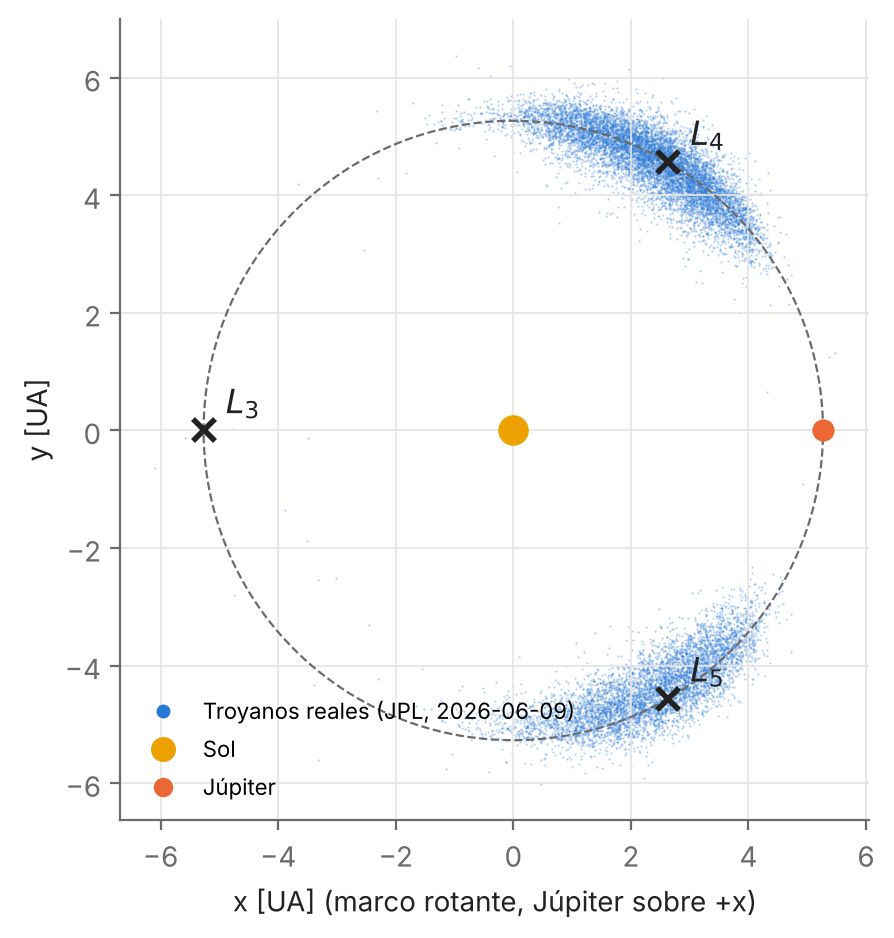
\includegraphics[width=\linewidth]{fig1_marco_rotante.png}\\
{\scriptsize 14\,809 troyanos reales, JPL, 9 jun 2026}
\end{columns}
\end{frame}

% 3 ------------------------------------------------------------------
\begin{frame}{Modelo: problema restringido de tres cuerpos en el marco rotante}
\begin{columns}[t]
\column{0.55\textwidth}
\textbf{Hipótesis}: Sol + Júpiter + asteroide sin masa. Unidades: $G(m_\odot+m_J)=1$, distancia $=1$, $n=1$.
\[
\mu=\frac{m_J}{m_\odot+m_J}=9{,}54\times10^{-4}
\]
\[
\mathcal L=\tfrac12\left[(\dot x-y)^2+(\dot y+x)^2\right]+\frac{1-\mu}{r_1}+\frac{\mu}{r_2}
\]
\[
\ddot x-2\dot y=\Omega_x,\qquad \ddot y+2\dot x=\Omega_y
\]
\column{0.42\textwidth}
\begin{itemize}
\item $-2\dot y$, $+2\dot x$: \textbf{Coriolis}.
\item $\mathcal L$ no depende de $t$ $\Rightarrow$ se conserva la constante de Jacobi
\[C_J=2\Omega-v^2\]
\item $L_4=(\tfrac12-\mu,\ \tfrac{\sqrt3}{2})$: triángulo equilátero.
\end{itemize}
\end{columns}
\end{frame}

% 4 ------------------------------------------------------------------
\begin{frame}{Teoría lineal alrededor de $L_4$}
Perturbamos $x=x_{L4}+\xi$, $y=y_{L4}+\eta$, con $\xi,\eta\propto e^{\lambda t}$:
\[
\lambda^4+\lambda^2+\tfrac{27}{4}\mu(1-\mu)=0
\quad\Rightarrow\quad
\omega_\pm^2=\tfrac12\left[1\pm\sqrt{1-27\mu(1-\mu)}\right]
\]
\begin{columns}[t]
\column{0.48\textwidth}
\begin{itemize}
\item Estable si $\mu<0{,}0385$ (Routh). Júpiter: \checkmark
\item Modo rápido: epiciclo, $11{,}9$ años.
\item Modo lento: \textbf{libración}
\[ T_{\rm lin}=\frac{2\pi}{\omega_-}\approx\frac{T_J}{\sqrt{27\mu/4}}=\boxed{147{,}4\ \text{años}} \]
\end{itemize}
\column{0.48\textwidth}
\begin{alertblock}{Tres predicciones comprobables}
\begin{enumerate}
\item El período \textbf{no} depende de la amplitud.
\item La libración es \textbf{simétrica} alrededor de $60^\circ$.
\item La única escala es $\mu$.
\end{enumerate}
\end{alertblock}
\end{columns}
\end{frame}

% 5 ------------------------------------------------------------------
\begin{frame}{Cómo lo pusimos a prueba}
\begin{enumerate}
\item \textbf{Barrido en amplitud} (PR3C plano completo): integración numérica DOP853 desde $\varphi_0=59^\circ$ hasta $23{,}5^\circ$.\\
Medimos amplitud $D$ y período de $\varphi=\lambda-\lambda_J$.
\item \textbf{Modelo promediado} (método independiente): péndulo no lineal
\[\ddot\varphi=-3\mu n^2\sin\varphi\left[1-(2-2\cos\varphi)^{-3/2}\right]\]
período por cuadratura.
\item \textbf{Troyanos reales}: 14\,809 asteroides (JPL SBDB, todos en la época 9 jun 2026) + Júpiter de JPL Horizons.\\
Problema restringido \textbf{3D}, Júpiter \textbf{circular} y \textbf{elíptico} ($e_J=0{,}048$), 2000 años.
\end{enumerate}
\end{frame}

% 6 ------------------------------------------------------------------
\begin{frame}{¿Por qué creerle al código? Verificaciones independientes}
\centering\small
\begin{tabular}{ll}
\toprule
Prueba & Resultado\\\midrule
Conservación de $C_J$ (barrido) & $|\Delta C_J/C_J|<7\times10^{-13}$\\
Conservación de $C_J$ (3D, 1500 años) & mediana $9\times10^{-6}$\\
Límite $D\to0$ & $T_{\rm num}=12{,}436\,T_J$ vs.\ $T_{\rm lin}=12{,}428\,T_J$ (0,06\,\%)\\
Dos métodos: completo vs.\ promediado & $<0{,}5\,\%$ hasta $D\approx40^\circ$\\
Convergencia: paso $T_J/300$ vs.\ $T_J/600$ & $\Delta D<0{,}12^\circ$, $\Delta T\sim0{,}01\,\%$\\
Dos integradores: RK4 vs.\ DOP853 & $\Delta D<0{,}02^\circ$, $\Delta T<0{,}02\,\%$\\
Elementos $\to$ estado $\to$ elementos & error $10^{-14}$\\
\bottomrule
\end{tabular}
\vspace{0.4cm}

Los errores numéricos son mucho menores que los efectos físicos que reportamos (1--10\,\%).
\end{frame}

% 7 ------------------------------------------------------------------
\begin{frame}{Resultado 1: el período deja de ser constante}
\begin{columns}[c]
\column{0.6\textwidth}
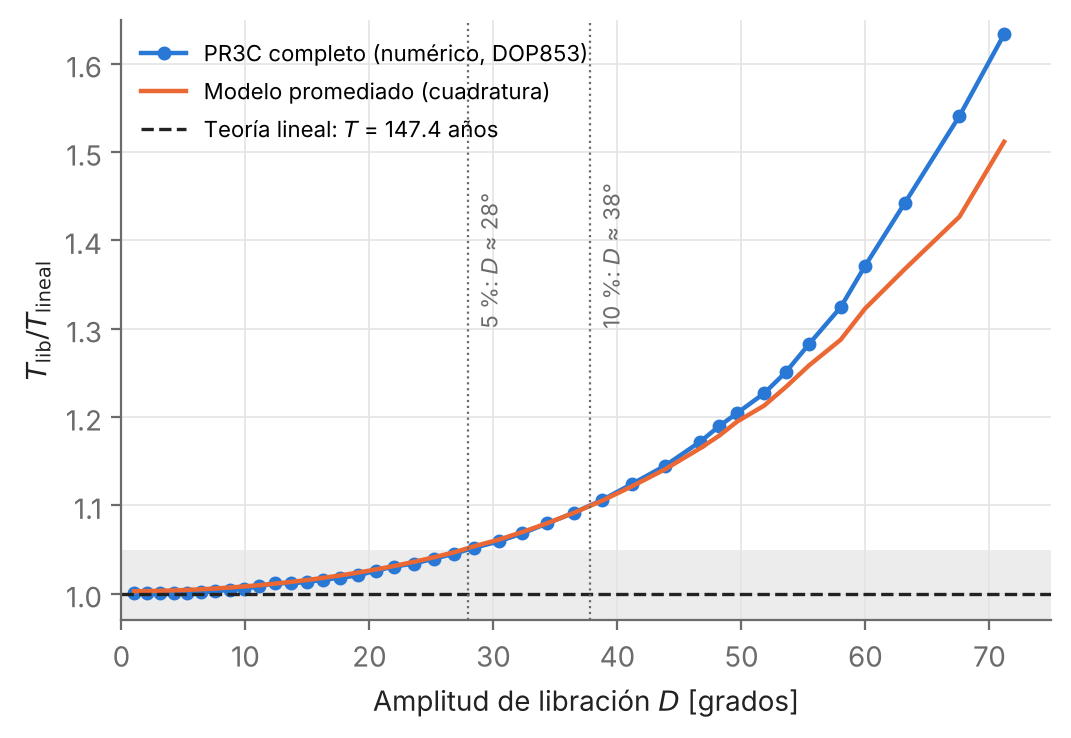
\includegraphics[width=\linewidth]{fig2_periodo_amplitud.png}
\column{0.38\textwidth}
\begin{itemize}
\item $D\to0$: se recupera $T_{\rm lin}$.
\item Corrección $\propto D^2$ (como en un péndulo).
\item Error del período lineal:
\begin{itemize}
\item \textbf{1\,\%} en $D\approx12^\circ$
\item \textbf{5\,\%} en $D\approx28^\circ$
\item \textbf{10\,\%} en $D\approx38^\circ$
\end{itemize}
\item Renacuajo máximo: $D\approx71^\circ$. Después, herradura.
\end{itemize}
\end{columns}
\end{frame}

% 8 ------------------------------------------------------------------
\begin{frame}{Resultado 2: antes que el período falla la forma}
\begin{columns}[c]
\column{0.58\textwidth}
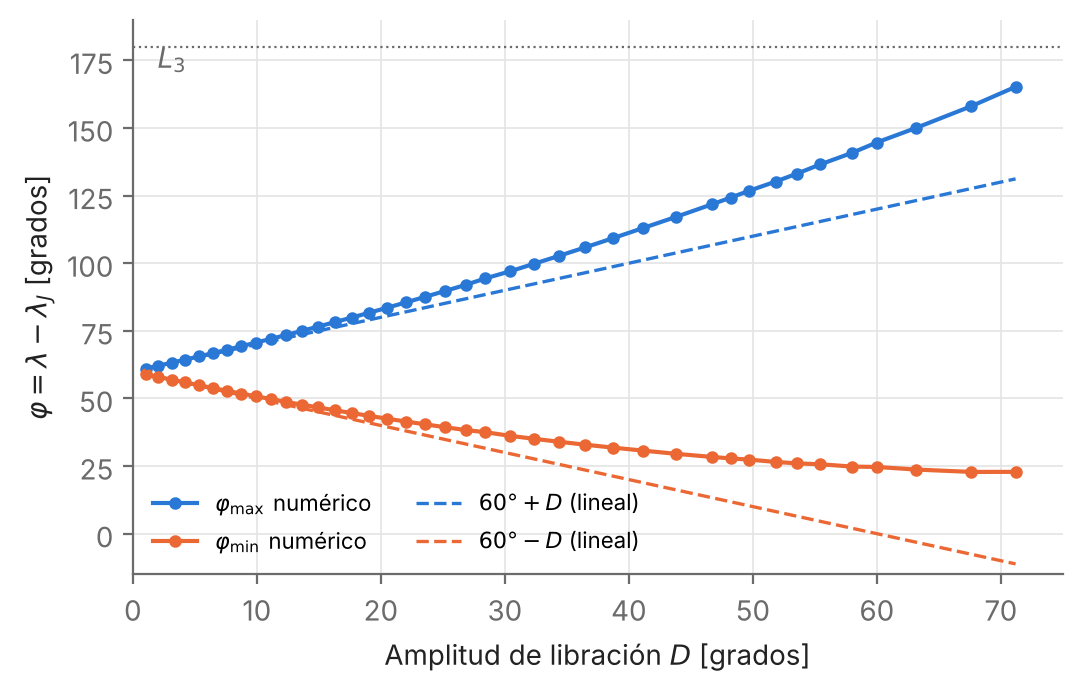
\includegraphics[width=\linewidth]{fig3_asimetria.png}
\column{0.4\textwidth}
\begin{itemize}
\item Lineal: $\varphi$ entre $60^\circ\pm D$.
\item Real: se estira hacia $L_3$ y se comprime frente a Júpiter.
\item Asimetría visible desde $D\approx11^\circ$.
\item Con $D=30^\circ$: $\varphi_{\max}=97^\circ$, no $90^\circ$.
\end{itemize}
\vspace{0.2cm}
\alert{Júpiter empuja más fuerte cuando el asteroide se acerca.}
\end{columns}
\end{frame}

% 9 ------------------------------------------------------------------
\begin{frame}{Resultado 3: ¿dónde están los troyanos reales?}
\begin{columns}[c]
\column{0.6\textwidth}
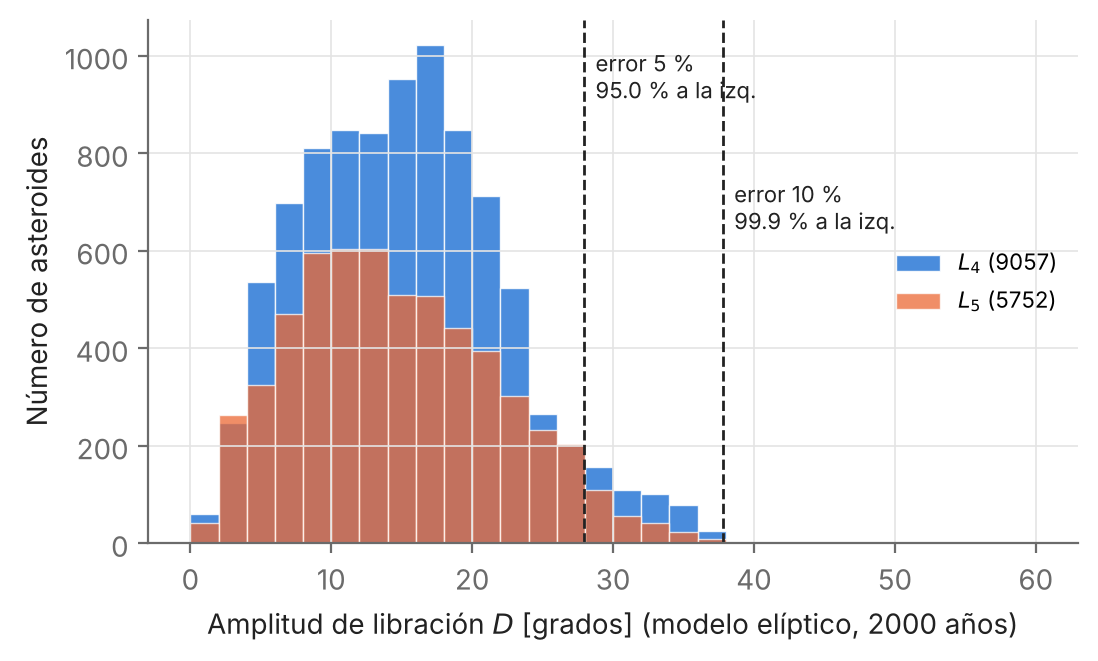
\includegraphics[width=\linewidth]{fig5_hist_amplitud.png}
\column{0.38\textwidth}
\begin{itemize}
\item $L_4$: 9\,057, $L_5$: 5\,752.
\item Amplitud mediana: $14{,}6^\circ$.
\item \textbf{95\,\%} tiene $D<28^\circ$ (error $<5\,\%$).
\item Solo 30 (0,2\,\%) escapan en 2000 años.
\end{itemize}
\vspace{0.2cm}
Por amplitud, casi todos son ``cuasi-lineales''.\\ \alert{¿Entonces la teoría lineal funciona?}
\end{columns}
\end{frame}

% 10 -----------------------------------------------------------------
\begin{frame}{Resultado 4: la inclinación es el verdadero límite}
\begin{columns}[c]
\column{0.58\textwidth}
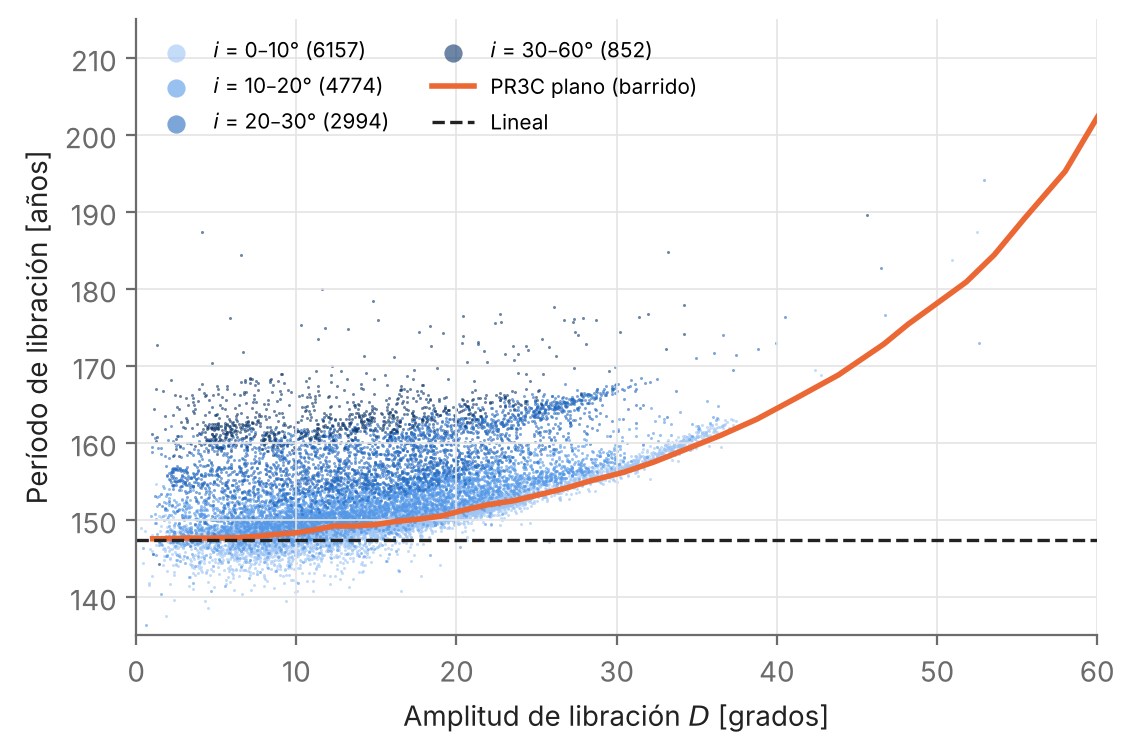
\includegraphics[width=\linewidth]{fig4_reales_T_vs_D.png}
\column{0.4\textwidth}
\begin{itemize}
\item Solo el \textbf{68\,\%} tiene un período a menos del 5\,\% del lineal (no el 95\,\%).
\item Con $D<10^\circ$:\\
$i<10^\circ$: 147,5 años\\
$i>30^\circ$: \textbf{162 años} (+10\,\%)
\item Un asteroide inclinado pasa tiempo fuera del plano de Júpiter: menos fuerza restauradora, libración más lenta.
\end{itemize}
\end{columns}
\end{frame}

% 11 -----------------------------------------------------------------
\begin{frame}{Dos troyanos reales frente a la teoría lineal}
\begin{columns}[c]
\column{0.6\textwidth}
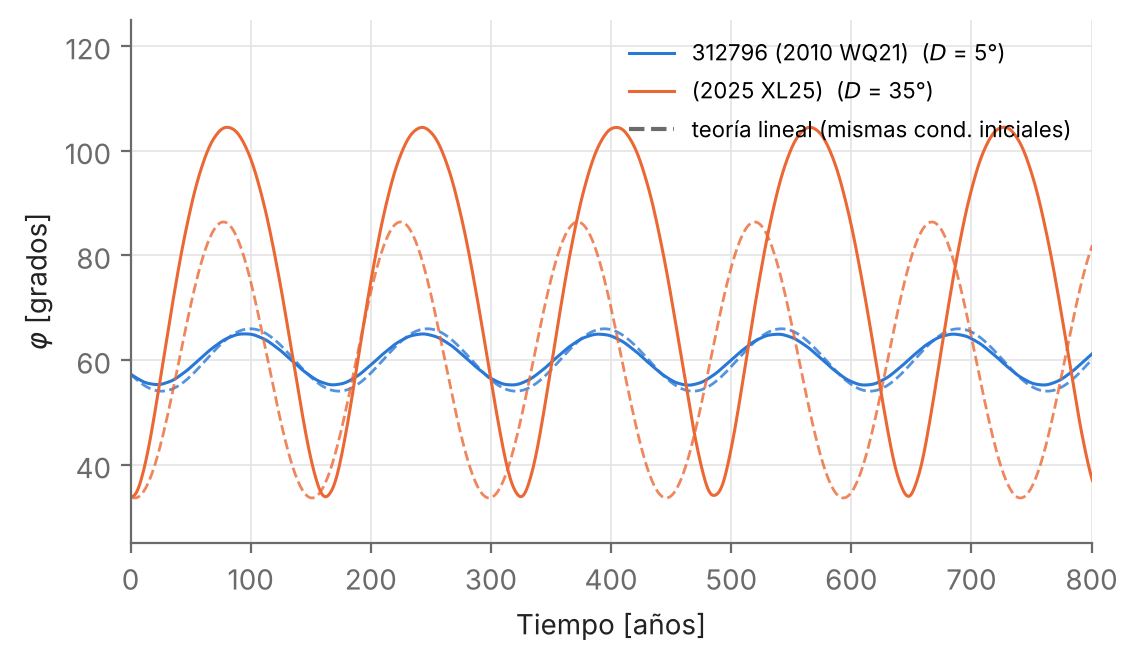
\includegraphics[width=\linewidth]{fig6_ejemplos.png}
\column{0.38\textwidth}
\begin{itemize}
\item Línea discontinua: solución lineal con las \textbf{mismas condiciones iniciales}.
\item $D=5^\circ$: casi perfecta.
\item $D=35^\circ$: máximo errado por $\sim18^\circ$, período 162 vs.\ 147 años, medio ciclo de desfase en 800 años.
\end{itemize}
\end{columns}
\end{frame}

% 12 -----------------------------------------------------------------
\begin{frame}{Una firma no lineal en los datos y una hipótesis cambiada}
\begin{columns}[t]
\column{0.48\textwidth}
\textbf{Centro de los enjambres (catálogo, sin simular)}
\begin{itemize}
\item $L_4$: $63{,}06^\circ\pm0{,}13^\circ$
\item $L_5$: $62{,}38^\circ\pm0{,}17^\circ$
\item Lineal: $60^\circ$. Modelo no lineal: $63{,}2^\circ$ / $62{,}4^\circ$ \checkmark
\end{itemize}
Es la asimetría del Resultado 2, vista en la población real.
\column{0.5\textwidth}
\textbf{Circular $\to$ elíptico} ($e_J=0{,}048$)\\[4pt]
\small
\begin{tabular}{lc}
\toprule
Cambio & Efecto en $T$\\\midrule
$e_J: 0\to0{,}048$ & 0,4\,\%\\
$D: 5^\circ\to28^\circ$ & 5\,\%\\
$i: <10^\circ\to>30^\circ$ & 10\,\%\\
\bottomrule
\end{tabular}\\[4pt]
\normalsize La excentricidad de Júpiter es lo \textbf{menos} importante.
\end{columns}
\end{frame}

% 13 -----------------------------------------------------------------
\begin{frame}{Conclusiones}
\begin{enumerate}
\item La teoría lineal ($T_{\rm lin}=147{,}4$ años) se recupera exactamente para $D\to0$ (verificado con dos métodos y con $C_J$).
\item Límite cuantitativo: el período falla un 5\,\% en $D\approx28^\circ$. La \textbf{forma} falla antes ($D\approx11^\circ$), y eso se ve en los datos: enjambres centrados en $\approx63^\circ$.
\item El 95\,\% de los troyanos reales tiene amplitud ``lineal'', pero solo el 68\,\% tiene período ``lineal'': \alert{la inclinación impone el límite antes que la amplitud.}
\item La excentricidad de Júpiter es un efecto menor ($<1\,\%$).
\end{enumerate}
\begin{block}{Respuesta}
El análisis lineal describe cuantitativamente (error $<5\,\%$) los troyanos con $D\lesssim25^\circ$ e $i\lesssim15^\circ$. Para el resto, solo da el orden de magnitud.
\end{block}
\end{frame}

% 14 -----------------------------------------------------------------
\begin{frame}{Limitaciones y siguientes pasos}
\begin{itemize}
\item No incluimos Saturno: su cercanía a la resonancia 5:2 con Júpiter controla la estabilidad en millones de años.
\item 2000 años de integración: estudiamos la libración, no la estabilidad de largo plazo.
\item Siguiente paso: teoría lineal en 3D para predecir analíticamente el efecto de la inclinación.
\item Comparar nuestras amplitudes con las amplitudes propias publicadas (AstDyS).
\end{itemize}
\vspace{0.6cm}
\centering\Large ¡Gracias!
\end{frame}

\end{document}
